\documentclass[10pt]{article}
\usepackage[margin=1in]{geometry}
\usepackage[T1]{fontenc}
\usepackage{lmodern}
\usepackage{microtype}
\usepackage{amsmath,amssymb}
\usepackage{booktabs,graphicx,array}
\usepackage{xcolor}
\usepackage{enumitem}
\usepackage{placeins}
\usepackage[font=small,labelfont=bf]{caption}
\usepackage[colorlinks=true,linkcolor=black,urlcolor=blue!50!black]{hyperref}
\setlist{itemsep=2pt,topsep=4pt,leftmargin=*}
\newcommand{\nctx}{365}
\newcommand{\neone}{2,500}
\newcommand{\exactDSFlash}{98}
\newcommand{\bestmodel}{DeepSeek V4 Flash}
\newcommand{\tiedwithbest}{DeepSeek V4 Pro}
\newcommand{\nsigbelow}{three}
\newcommand{\deltamin}{7}
\newcommand{\deltamax}{17}
\newcommand{\exactmin}{81}
\newcommand{\exactmax}{98}
\newcommand{\recallmin}{0.966}
\newcommand{\recallmax}{0.996}
\newcommand{\otherswrong}{25}
\newcommand{\othersmadeup}{0}
\newcommand{\flashmadeup}{1,032}
\newcommand{\flashworstmade}{991}
\newcommand{\flashworstgold}{100}
\newcommand{\medianmissed}{1}
\newcommand{\ninvalid}{7}
\newcommand{\nrefused}{2}
\newcommand{\failDSPro}{4}
\newcommand{\failDSFlash}{2}
\newcommand{\largeHaiku}{53}
\newcommand{\largeMiMoFlash}{34}
\newcommand{\nenum}{100}
\newcommand{\smallmin}{93}
\newcommand{\orpooledanswer}{0.50}
\newcommand{\orpooledanswerci}{0.36--0.60}
\newcommand{\orpooledtable}{0.39}
\newcommand{\orpooledtableci}{0.22--0.56}
\newcommand{\fmtMiMoFlashJson}{86}
\newcommand{\fmtMiMoFlashNl}{73}
\newcommand{\condsizeone}{13}
\newcommand{\condsizetwo}{6.5}
\newcommand{\condsizethree}{3.5}
\newcommand{\ragrecall}{0.869 for all models}
\newcommand{\nscalar}{35}
\newcommand{\scalarerrors}{11}
\newcommand{\scalarunder}{9}
\newcommand{\rsmallDSPro}{1,050}
\newcommand{\rlargeDSPro}{8,832}
\newcommand{\rsmallHaiku}{173}
\newcommand{\rlargeHaiku}{6,442}
\newcommand{\flashshallowexact}{62}
\newcommand{\flashdeepexact}{72}
\newcommand{\etwonote}{DeepSeek V4 Pro's E2 runs are pending (provider usage limits).}
\newcommand{\agreemin}{87}
\newcommand{\agreemax}{100}
\newcommand{\flipmin}{0}
\newcommand{\flipmax}{13}
\newcommand{\reasonshare}{77--97}
\newcommand{\totalcalls}{3,796}
\newcommand{\failedcalls}{1,163}

\newcommand{\takeaway}[1]{\par\smallskip\noindent\textit{Takeaway: #1}\par}

\title{\textbf{Completeness of Relational Operations in Language Models}\\[3pt]
\large Results on a 500-Question Benchmark}
\author{Daryl Alfaro}
\date{\today}

\begin{document}
\maketitle

\begin{abstract}
We report results for five language models on a 500-question benchmark that asks for \emph{every} item
satisfying a condition, over records whose exact answers are obtained by executing SQL. On the \nctx{}
questions whose records are in the prompt, mean recall is \recallmin--\recallmax, but only \exactmin--\exactmax\%
of answers are exactly the correct set, and nearly all errors are omitted items. For three models the chance of a
complete answer falls significantly as the number of correct items grows. Alternative prompts did not improve
completeness. Models that stayed complete used far more reasoning tokens on larger answer sets.
\end{abstract}

\section{Process}
\paragraph{Benchmark.} The benchmark has 500 questions over \ntables{} synthetic tables (\nrecords{} records)
about fictional entities, so answers cannot come from memory. Each question is generated with the SQL query that
defines it, and its gold answer is that query's result in SQLite. The 400 \emph{in-context} questions put all
records in the prompt; 60 \emph{memory-only} questions filter fixed lists (U.S.\ states, chemical elements,
presidents' surnames); 40 \emph{retrieval} questions supply the top-$k$ BM25 results. For in-context enumeration,
exactly $g\in\{5,10,20,50,100\}$ of $n\in\{50,200,500,1000\}$ rows match, so answer size and table size vary
independently. Table~\ref{tab:composition} lists the slices.

\paragraph{Models.} DeepSeek V4 Pro and V4 Flash (OpenCode Go API), Claude Haiku 5.5 (Claude Code CLI
\claudecli, no tools) and MiMo-V2.6 Pro and Flash (OpenRouter), each with its default reasoning, temperature~0
where supported, and a 32{,}768-token output limit. Answers are returned as JSON.

\paragraph{Metrics.} For gold set $G$ and predicted set $P$: recall $|P\cap G|/|G|$, precision $|P\cap G|/|P|$,
and \textbf{exact-set accuracy} $\mathbb{1}[P=G]$, the primary measure. Each error is classified as
\emph{missing}, \emph{near-miss} (a garbled copy of a missing item), \emph{wrong} (in the data but not
qualifying), \emph{made-up} (not in the data) or \emph{duplicate}. An answer \emph{omits} if it misses a correct
item and \emph{commits} if it adds an incorrect one.

\paragraph{Runs and statistics.} \textbf{E1}: all 500 questions, direct prompt. \textbf{E2}: a stratified
100-question subset with a ``be exhaustive'' prompt and a ``check every record first'' prompt. \textbf{E3}: the
subset again with the direct prompt. Intervals are 95\% (Wilson for proportions, question-level bootstrap for
means); model and prompt comparisons use paired question-level differences; trends with answer size use a
logistic regression on $\log_2$ of the number of correct items.

\begin{table}[!htbp]
\centering\small
\resizebox{\linewidth}{!}{\begin{tabular}{lrlrr}
\toprule
Slice & Qs & Variants & Answer size & Context (k tok.) \\
\midrule
Enumeration & 100 & one category filter & 5--100 & 7.6 \\
Enumeration (memory only) & 60 & U.S. states, elements, presidents & 2--50 & 0.0 \\
Enumeration (retrieval) & 40 & BM25 top-$k$, $k\in\{10,20,50\}$ & 5--40 & 1.1 \\
\midrule
Selection & 60 & 1--3 conditions & 1--92 & 4.1 \\
Projection & 40 & DISTINCT; 2--3 attributes & 7--39 & 2.9 \\
JOIN & 60 & 1:1, 1:N, M:N & 3--55 & 3.4 \\
Aggregation & 50 & COUNT, SUM, MIN/MAX/AVG, GROUP BY & 3--367 & 2.8 \\
Nested query & 40 & IN, NOT IN, correlated, scalar & 3--32 & 2.7 \\
Set operation & 50 & UNION, INTERSECT, EXCEPT, 3-way & 4--97 & 0.7 \\
\bottomrule
\end{tabular}
}
\caption{Benchmark composition. Answer size is the number of correct items (for aggregation, records
aggregated); context is the median data size in the prompt.}
\label{tab:composition}
\end{table}

\FloatBarrier
\section{Results}

\FloatBarrier
\subsection{Overall completeness}
Table~\ref{tab:main} shows the \nctx{} in-context set-valued questions. Recall and precision are close to 1 for
every model, but exact-set accuracy ranges from \exactmax\% to \exactmin\%. The two DeepSeek models are tied; the
other three are significantly below the best model, by 7 to 17 percentage points.

\begin{table}[!htbp]
\centering\small
\resizebox{\linewidth}{!}{\begin{tabular}{lrrrrrrr}
\toprule
Model & Exact-set acc.\ (\%) & $\Delta$ vs.\ best (pp) & Mean recall & Mean prec. & Omit.\ (\%) & Comm.\ (\%) & Invalid \\
\midrule
DeepSeek V4 Pro & 98 [96, 99] & $-0.3$ [-2.5, +1.6] & 0.996 [0.991, 1.000] & 1.000 & 2 & 0 & 1 \\
DeepSeek V4 Flash & 98 [96, 99] & (reference) & 0.996 [0.989, 1.000] & 0.999 & 1 & 1 & 1 \\
Claude Haiku 5.5 & 91 [88, 93] & $-7.1$ [-10.1, -4.1] & 0.995 [0.993, 0.997] & 0.999 & 9 & 1 & 0 \\
MiMo-V2.6 Pro & 90 [86, 93] & $-8.2$ [-11.8, -4.9] & 0.987 [0.978, 0.994] & 0.997 & 7 & 4 & 2 \\
MiMo-V2.6 Flash & 81 [77, 85] & $-16.7$ [-20.8, -12.3] & 0.966 [0.952, 0.979] & 0.976 & 15 & 10 & 2 \\
\bottomrule
\end{tabular}
}
\caption{In-context set-valued questions (E1, $n=\nctx$ per model), with 95\% intervals. $\Delta$: paired
difference in exact-set accuracy from the best model. \emph{Omit.}/\emph{Comm.}: share of answers that omit a
correct item / add an incorrect or duplicate one.}
\label{tab:main}
\end{table}

\begin{figure}[!htbp]
\centering
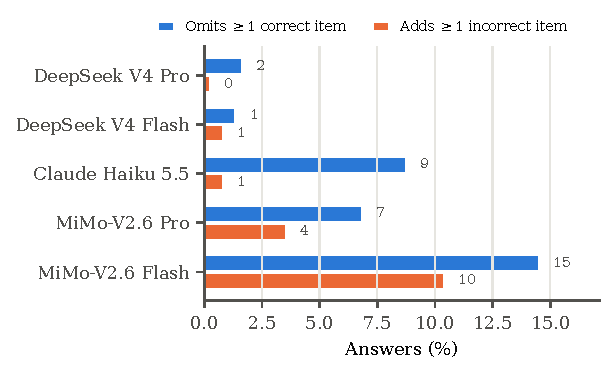
\includegraphics[width=0.58\linewidth]{generated/error_profile.pdf}
\caption{Share of in-context answers that omit at least one correct item, and that add at least one incorrect
item (E1).}
\label{fig:errors}
\end{figure}

Errors are almost all omissions (Figure~\ref{fig:errors}; counts in Table~\ref{tab:errors}). Four models together
returned \otherswrong{} wrong items and \othersmadeup{} made-up items across all their answers. MiMo-V2.6 Flash
is the exception: it returned \flashmadeup{} made-up items, \flashworstmade{} of them on a single
\flashworstgold-item question.
\takeaway{high recall does not mean complete answers; models leave correct items out far more often than they add
wrong ones, so incompleteness is not visible in what they list.}

\FloatBarrier
\subsection{Completeness and answer size}
On in-context enumeration (Figure~\ref{fig:size}, Table~\ref{tab:trend}), every model is complete on at least
93\% of questions with up to 10 correct items. With 50 or more, Claude Haiku 5.5 falls to \largeHaiku\%,
MiMo-V2.6 Pro to \largeMiMoPro\% and MiMo-V2.6 Flash to \largeMiMoFlash\%. The decline is significant for DeepSeek
V4 Pro, Claude Haiku 5.5 and MiMo-V2.6 Flash, whose odds of a complete answer fall to 0.31--0.41$\times$ per
doubling of the answer set. DeepSeek V4 Flash fails too rarely to show a trend.
\takeaway{the more items a correct answer contains, the less likely it is to be complete.}

\begin{figure}[!htbp]
\centering
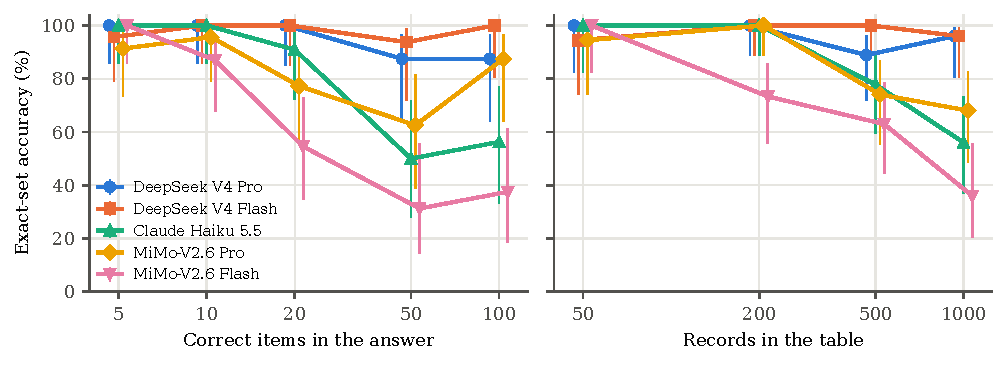
\includegraphics[width=\linewidth]{generated/size_curves.pdf}
\caption{In-context enumeration (E1): exact-set accuracy by number of correct items (left) and table size (right),
with 95\% Wilson intervals.}
\label{fig:size}
\end{figure}

\begin{table}[!htbp]
\centering\small
\begin{tabular}{lrrrrr}
\toprule
Model & $\leq$10 items (\%) & $\geq$50 items (\%) & Failures & OR: answer size [95\% CI] & OR: table size [95\% CI] \\
\midrule
DeepSeek V4 Pro & 100 & 88 & 4 & n.e. & n.e. \\
DeepSeek V4 Flash & 98 & 97 & 2 & n.e. & n.e. \\
Claude Haiku 5.5 & 100 & 53 & 17 & 0.17 [0.02, 0.28] & 0.07 [0.01, 0.17] \\
MiMo-V2.6 Pro & 93 & 75 & 16 & 0.79 [0.44, 1.20] & 0.44 [0.11, 0.76] \\
MiMo-V2.6 Flash & 93 & 34 & 34 & 0.33 [0.15, 0.44] & 0.29 [0.08, 0.45] \\
\midrule
\textit{All models (pooled)} & 97 & 69 & 73 & 0.50 [0.36, 0.60] & 0.39 [0.22, 0.56] \\
\bottomrule
\end{tabular}

\caption{In-context enumeration (E1): exact-set accuracy for small and large answer sets, and the odds ratio of a
complete answer per doubling of the number of correct items (below 1 means degradation).}
\label{tab:trend}
\end{table}

\FloatBarrier
\subsection{By operation}
Every operation except set operations produced incomplete answers from at least three models
(Table~\ref{tab:operation}). Enumeration, which has the largest answer sets, is hardest; set operations are
solved almost perfectly.
\takeaway{the effect is not specific to one operation.}

\begin{table}[!htbp]
\centering\small
\resizebox{\linewidth}{!}{\begin{tabular}{lrrrrrr}
\toprule
Operation & Qs & DeepSeek\ V4\ Pro & DeepSeek\ V4\ Flash & Claude\ Haiku\ 5.5 & MiMo-V2.6\ Pro & MiMo-V2.6\ Flash \\
\midrule
Enumeration & 100 & 96 & 98 & 83 & 84 & 66 \\
Selection & 60 & 97 & 98 & 95 & 93 & 88 \\
Projection & 40 & 100 & 95 & 90 & 90 & 82 \\
JOIN & 60 & 100 & 98 & 93 & 88 & 82 \\
Aggregation & 15 & 93 & 93 & 93 & 87 & 67 \\
Nested query & 40 & 98 & 100 & 90 & 92 & 90 \\
Set operation & 50 & 100 & 100 & 100 & 98 & 100 \\
\bottomrule
\end{tabular}
}
\caption{Exact-set accuracy (\%) by operation, in-context set-valued questions (E1). Aggregation here is GROUP BY;
scalar aggregates are in Table~\ref{tab:scalar}.}
\label{tab:operation}
\end{table}

\FloatBarrier
\subsection{Memory-only and retrieval settings}
From memory, both DeepSeek models were always exact; the other three missed members of short fixed lists
(Table~\ref{tab:settings}), e.g.\ Claude Haiku 5.5 named Kentucky but not New Jersey as a state ending in ``y''.
In the retrieval setting every model returned every correct record that was retrieved, so recall (0.869 for all)
equals the retriever's recall.
\takeaway{the retrieval slice, as built, measures the retriever rather than the models.}

\begin{table}[!htbp]
\centering\small
\resizebox{\linewidth}{!}{\begin{tabular}{lrrrr}
\toprule
Model & Memory: exact (\%) & Memory: recall & Retrieval: recall & Retrieval: recall over retrieved \\
\midrule
DeepSeek V4 Pro & 100 & 1.000 & 0.869 & 1.000 \\
DeepSeek V4 Flash & 100 & 1.000 & 0.869 & 1.000 \\
Claude Haiku 5.5 & 87 & 0.952 & 0.869 & 1.000 \\
MiMo-V2.6 Pro & 83 & 0.955 & 0.869 & 1.000 \\
MiMo-V2.6 Flash & 83 & 0.958 & 0.869 & 1.000 \\
\bottomrule
\end{tabular}
}
\caption{Memory-only and retrieval settings (E1).}
\label{tab:settings}
\end{table}

\FloatBarrier
\subsection{Scalar aggregation}
On \nscalar{} COUNT, SUM, MIN, MAX and AVG questions (Table~\ref{tab:scalar}), both DeepSeek models were always
exact. Of the other models' 11 errors, 9 were undercounts.
\takeaway{wrong totals are mostly too low, consistent with dropped items.}

\begin{table}[!htbp]
\centering\small
\begin{tabular}{lrrrr}
\toprule
Model & Qs & Exact (\%) & Under-counts & Over-counts \\
\midrule
DeepSeek V4 Pro & 35 & 100 & 0 & 0 \\
DeepSeek V4 Flash & 35 & 100 & 0 & 0 \\
Claude Haiku 5.5 & 35 & 94 & 2 & 0 \\
MiMo-V2.6 Pro & 35 & 91 & 3 & 0 \\
MiMo-V2.6 Flash & 35 & 83 & 4 & 2 \\
\bottomrule
\end{tabular}

\caption{Scalar aggregation questions (E1).}
\label{tab:scalar}
\end{table}

\FloatBarrier
\subsection{Consistency across runs}
Two independent samples of the subset agreed on 87--100\% of verdicts (Table~\ref{tab:repeats}). Of 13 failures
re-run three times each (Table~\ref{tab:cases}), some recurred every time: Claude Haiku 5.5's missing U.S.\
states, and DeepSeek V4 Pro's and MiMo-V2.6 Flash's misses on the same 50-item list. When MiMo-V2.6 Pro failed
on that list it omitted the same three employees each time. Others, including Claude Haiku 5.5's misses on
selection, JOIN, projection and COUNT questions, never recurred.
\takeaway{some failures are systematic, but many are run-to-run variation, so completeness is best reported as a
rate over many questions.}

\begin{table}[!htbp]
\centering\small
\begin{tabular}{lrrr}
\toprule
Model & Qs & Same verdict (\%) & Questions that flipped \\
\midrule
DeepSeek V4 Pro & 87 & 98 [92, 99] & 2 \\
DeepSeek V4 Flash & 93 & 100 [96, 100] & 0 \\
Claude Haiku 5.5 & 93 & 94 [87, 97] & 6 \\
MiMo-V2.6 Pro & 93 & 91 [84, 96] & 8 \\
MiMo-V2.6 Flash & 93 & 87 [79, 92] & 12 \\
\bottomrule
\end{tabular}

\caption{Agreement between two independent samples of the direct prompt (E1 vs.\ E3), with 95\% Wilson
intervals.}
\label{tab:repeats}
\end{table}

\begin{table}[!htbp]
\centering\small
\resizebox{\linewidth}{!}{\begin{tabular}{llrrp{5.2cm}c}
\toprule
Model & Question & Answers & Records & Main-run outcome & Reproduced \\
\midrule
Claude Haiku 5.5 & \texttt{enum-par-013} & 2 & 50 & recall 0.50, 1 missing & 2/3 \\
Claude Haiku 5.5 & \texttt{enum-par-021} & 11 & 50 & recall 0.73, 3 missing & 3/3 \\
Claude Haiku 5.5 & \texttt{sel-029} & 13 & 400 & recall 0.85, 2 missing & 0/3 \\
Claude Haiku 5.5 & \texttt{join-004} & 55 & 100 & recall 0.93, 4 missing & 0/3 \\
Claude Haiku 5.5 & \texttt{nest-022} & 13 & 200 & recall 0.92, 1 missing & 2/3 \\
Claude Haiku 5.5 & \texttt{proj-031} & 37 & 300 & recall 0.89, 4 missing & 0/3 \\
Claude Haiku 5.5 & \texttt{agg-015} & 12 & 400 & answered 11 (gold 12) & 0/3 \\
Claude Haiku 5.5 & \texttt{enum-ctx-029} & 50 & 500 & recall 0.96, 2 missing & 0/3 \\
DeepSeek V4 Pro & \texttt{enum-ctx-029} & 50 & 500 & recall 0.98, 1 missing & 3/3 \\
MiMo-V2.6 Flash & \texttt{enum-ctx-029} & 50 & 500 & recall 0.94, 3 missing, 3 wrong & 2/3* \\
MiMo-V2.6 Pro & \texttt{enum-ctx-029} & 50 & 500 & recall 0.92, 4 missing & 1/3 \\
MiMo-V2.6 Flash & \texttt{enum-ctx-035} & 100 & 1000 & recall 0.52, 46 missing, 2 near-miss, 19 wrong, 371 made-up, 34 duplicate & 2/3 \\
DeepSeek V4 Flash & \texttt{enum-ctx-018} & 5 & 50 & recall 0.80, 1 near-miss & 0/3 \\
\bottomrule
\end{tabular}
}
\caption{Selected failures, each re-run three more times on the same model. \emph{Reproduced}: re-runs again not
exactly correct (* marks a re-run with no parseable answer, not counted). MiMo cases come from an earlier
OpenCode Go run of the same models; DeepSeek and MiMo re-runs used OpenRouter.}
\label{tab:cases}
\end{table}

\FloatBarrier
\subsection{Prompt variants}
Neither the ``be exhaustive'' nor the ``check every record'' prompt changed exact-set accuracy significantly for
any model; every paired interval includes zero (Table~\ref{tab:prompting}).
\takeaway{simple prompting does not fix incompleteness.}

\begin{table}[!htbp]
\centering\small
\begin{tabular}{lrrrr}
\toprule
Model & Qs & Exhaustive $-$ direct (pp) & Qs & Row-by-row $-$ direct (pp) \\
\midrule
DeepSeek V4 Pro & -- & -- & -- & -- \\
DeepSeek V4 Flash & 93 & $-2.2$ [-5.4, +0.0] & 93 & $+0.0$ [+0.0, +0.0] \\
Claude Haiku 5.5 & 93 & $+1.1$ [-3.2, +5.4] & 93 & $-2.2$ [-6.5, +2.2] \\
MiMo-V2.6 Pro & 93 & $+1.1$ [-5.4, +6.5] & 93 & $+4.3$ [-1.1, +9.7] \\
MiMo-V2.6 Flash & 93 & $+0.0$ [-8.6, +8.6] & 93 & $+6.5$ [-2.2, +15.1] \\
\bottomrule
\end{tabular}

\caption{Paired change in exact-set accuracy (percentage points) from the direct prompt on the subset (E2), with
95\% bootstrap intervals. DeepSeek V4 Pro's E2 runs did not finish within its provider's usage limits.}
\label{tab:prompting}
\end{table}

\FloatBarrier
\subsection{Reasoning effort}
Median reasoning length rose with answer size for the models that stayed complete
(Figure~\ref{fig:reasoning}): from \rsmallDSPro{} to \rlargeDSPro{} tokens for DeepSeek V4 Pro and from
\rsmallHaiku{} to \rlargeHaiku{} for Claude Haiku 5.5. MiMo-V2.6 Flash often answered after one sentence of
reasoning; its \flashshallown{} answers with under 100 reasoning tokens were complete \flashshallowexact\% of the
time, against \flashdeepexact\% for the rest.
\takeaway{completeness on large answer sets coincides with much longer reasoning; this is an association, not a
controlled result.}

\begin{figure}[!htbp]
\centering
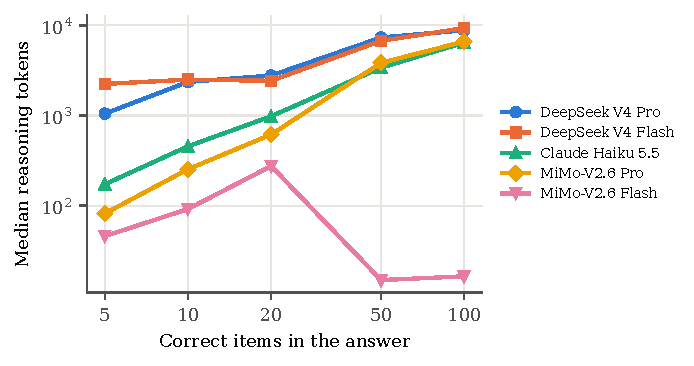
\includegraphics[width=0.6\linewidth]{generated/reasoning.pdf}
\caption{Median reasoning tokens on in-context enumeration by number of correct items (E1).}
\label{fig:reasoning}
\end{figure}

\FloatBarrier
\subsection{Usage}
Across all runs the five models made \totalcalls{} calls; \reasonshare\% of output tokens were reasoning
(Table~\ref{tab:usage}).

\begin{table}[!htbp]
\centering\footnotesize\setlength{\tabcolsep}{4pt}
\begin{tabular}{lrrrrrr}
\toprule
Model & Calls & Input (M) & Output (M) & of which reasoning (M) & Cost (USD) & Median latency (s) \\
\midrule
DeepSeek V4 Pro & 1021 & 3.83 & 2.21 & 2.14 & 6.87 & 23.43 \\
DeepSeek V4 Flash & 1307 & 5.08 & 3.02 & 2.81 & 2.52 & 12.48 \\
Haiku 5.5 & 893 & 8.04 & 1.88 & 1.64 & 2.49 & 7.70 \\
MiMo-V2.6 Pro & 800 & 5.77 & 2.00 & 1.78 & 3.29 & 16.65 \\
MiMo-V2.6 Flash & 800 & 5.78 & 1.72 & 1.32 & 1.25 & 13.10 \\
\bottomrule
\end{tabular}

\caption{Usage across all experiments, including retried calls. Input and output in millions of tokens;
\emph{Reasoning}: share of output tokens; cost at provider list prices (Claude Haiku 5.5 and the OpenCode Go
models were used through subscriptions); latency is the median per call.}
\label{tab:usage}
\end{table}

\FloatBarrier
\section{Summary}
\begin{itemize}
\item Mean recall of \recallmin--\recallmax{} corresponds to exact-set accuracy of only \exactmin--\exactmax\%;
\omitmin--\omitmax\% of in-context answers omit at least one correct item.
\item Errors are omissions, not additions, for four of five models; one model fabricates items on long lists.
\item Completeness falls with answer size, significantly for three models.
\item Prompt variants do not help; complete models reason far longer on large answer sets.
\item Caveats: synthetic data from one seed; one sample per question in E1 (0--13\% of verdicts change on a second
sample); the retrieval slice measures the retriever; DeepSeek V4 Pro lacks E2 results; a stopped Claude Haiku 4.5
run (90 questions) is excluded.
\end{itemize}
\noindent Code, data, raw responses and run manifests:\\
\url{https://github.com/daryl-888/llm-relational-completeness}.\\
Statistics follow E.~Miller, ``Adding Error Bars to Evals'' (2024), \url{https://arxiv.org/abs/2411.00640}.

\FloatBarrier
\clearpage
\appendix
\section{Additional results}

\begin{table}[!htbp]
\centering\small
\begin{tabular}{lrrrrr}
\toprule
Model & Missing & Near-miss & Wrong & Made-up & Duplicate \\
\midrule
DeepSeek V4 Pro & 16 & 0 & 1 & 0 & 0 \\
DeepSeek V4 Flash & 43 & 1 & 3 & 0 & 0 \\
Claude Haiku 5.5 & 75 & 0 & 6 & 0 & 0 \\
MiMo-V2.6 Pro & 104 & 0 & 15 & 0 & 0 \\
MiMo-V2.6 Flash & 492 & 7 & 311 & 1,032 & 316 \\
\bottomrule
\end{tabular}

\caption{Error counts by type on in-context set-valued questions (E1).}
\label{tab:errors}
\end{table}

\begin{figure}[!htbp]
\centering
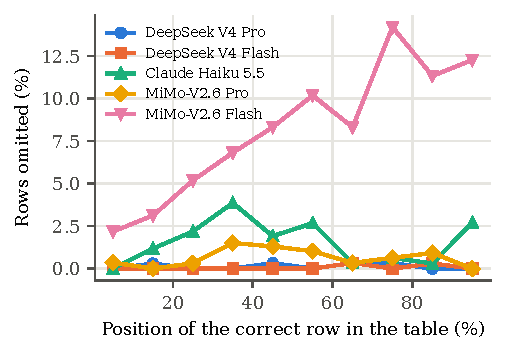
\includegraphics[width=0.58\linewidth]{generated/position.pdf}
\caption{Share of correct rows omitted by the row's position in the table (in-context enumeration, E1). MiMo-V2.6
Flash omits rows near the end more often; the other models omit too few rows for a clear pattern.}
\label{fig:position}
\end{figure}

\end{document}
